\documentclass[12pt, twoside]{article}
\usepackage[letterpaper, margin=1in, headsep=0.5in]{geometry}
\usepackage[english]{babel}
\usepackage[utf8]{inputenc}
\usepackage{amsmath}
\usepackage{amsfonts}
\usepackage{amssymb}
\usepackage{tikz}
\usetikzlibrary{quotes, angles}
\usepackage{graphicx}
\usepackage{enumitem}
\usepackage{multicol}

\newif\ifmeta
\metatrue %print standards and topics tags

\title{Regents Geometry}
\author{Chris Huson}
\date{September 2020}

\usepackage{fancyhdr}
\pagestyle{fancy}
\fancyhf{}
\renewcommand{\headrulewidth}{0pt} % disable the underline of the header
\raggedbottom


\fancyhead[LE]{\thepage}
\fancyhead[RO]{\thepage \\ Name: \hspace{4cm} \,\\}
\fancyhead[LO]{BECA / Dr. Huson / Geometry 07-Similarity\\* pset ID: 109}

\begin{document}

\subsubsection*{7-4bCW-Tangent}
\begin{enumerate}
\item Graph and label $\triangle ABC$ with $A(0,0)$, $B(4,7)$, and $C(4,0)$. Calculate each length:
  \begin{enumerate}[itemsep=1.25cm]  
  \begin{multicols}{2}
        \item $AC=$ \hfill (1 star)
        \item $BC=$ \hfill (1 star)
        \item $AB=\sqrt{AC^2+BC^2}$ \hfill (2 stars) \vspace{2cm}
  \begin{center}
    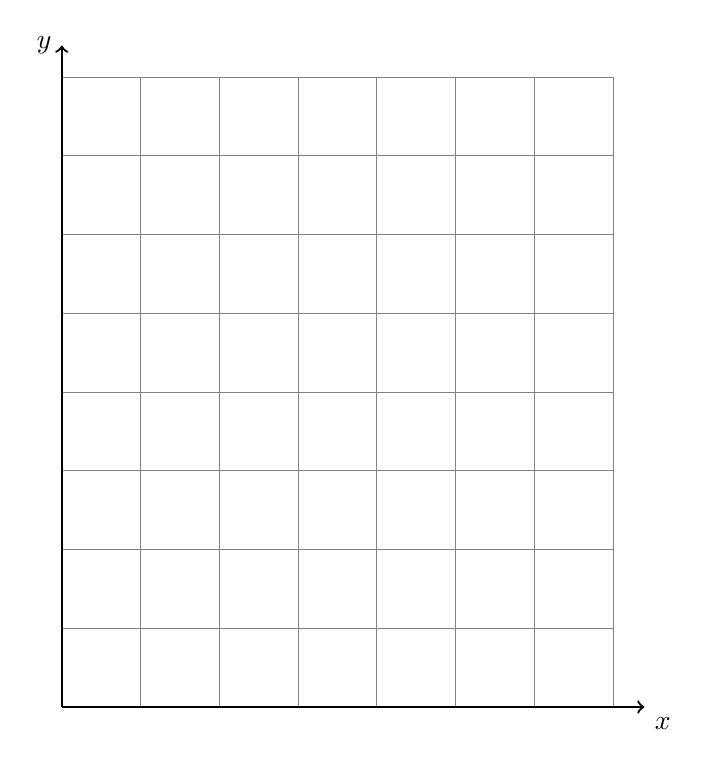
\begin{tikzpicture}%[scale=.635]
      \draw [help lines] (0,0) grid (7,8);
      \draw [thick, ->] (0,0) -- (7.4,0) node [below right] {$x$};
      \draw [thick, ->] (0,0)--(0,8.4) node [left] {$y$};
    \end{tikzpicture}
  \end{center}
  \end{multicols}\vspace{2cm}
    \item Use a protractor to measure $\angle BAC$ in degrees.  \hfill (1 star)
    \item The tangent of an angle is the ratio of the side lengths \emph{opposite} over \emph{adjacent} to the angle. Write down the value as a fraction.  \hfill (1 star)\\[0.5cm]
      $\tan \angle BAC=$
    \item Find $m\angle BAC$ with a calculator's inverse tangent function,\\ $\displaystyle m \angle BAC = \tan^{-1}(\frac{opp}{adj})$  \hfill (2 stars)
  \end{enumerate}

\newpage
\subsubsection*{Mastery topic: Calculator use}
\item Express the result to the nearest thousandth. \hfill (1 star each) \vspace{.5cm}
    \begin{multicols}{2}
      \begin{enumerate}
        \item $\tan 22^\circ = $ \vspace{1cm}
        \item $\tan 81^\circ =$
        \item $\tan 15^\circ = $ \vspace{1cm}
        \item $\tan 65^\circ =$
      \end{enumerate}
    \end{multicols} \vspace{1cm}

\item Round each value to the nearest degree. \hfill (1 star each) \vspace{.5cm}
    \begin{multicols}{2}
      \begin{enumerate}
        \item $\tan^{-1} (2) = $ \vspace{1cm}
        \item $\tan^{-1} (0.5) =$
        \item $\tan^{-1} (1) = $ \vspace{1cm}
        \item $\tan^{-1} (\sqrt{3}) =$
      \end{enumerate}
    \end{multicols} \vspace{1cm}

\subsubsection*{Mastery topic: Modeling. Do Not Solve}
\item Given right $\triangle JKL$ with $\overline{JK} \perp \overline{KL}$, $JK=11$, $m\angle J=18^\circ$. (mark the diagram)\\[0.5cm]
    Let $x$ be the length of the side opposite $\angle J$, $x=KL$. Write an equation expressing $\tan \angle J$ as a ratio of \emph{opposite} over \emph{adjacent}. \hfill (2 stars)
      \begin{flushright}
          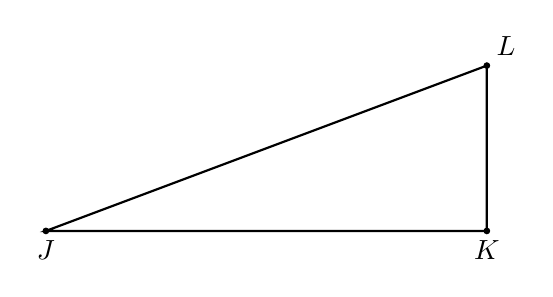
\begin{tikzpicture}[scale=0.7]
            \draw [thick](-1,0)--(7,0)--(7,3)--cycle;
            \draw [fill] (-1,0) circle [radius=0.05] node[below]{$J$};
            \draw [fill] (7,0) circle [radius=0.05] node[below]{$K$};
            \draw [fill] (7,3) circle [radius=0.05] node[above right]{$L$};
          \end{tikzpicture}
        \end{flushright}

\newpage
\item Given right $\triangle ABC$ with $m\angle C =90^\circ$, $BC=5$, $m\angle A=38^\circ$. (mark the diagram)\\[0.5cm]
  Let $x$ be the length of the side adjacent to $\angle A$, $x=AC$. Write an equation expressing $\tan \angle A$ as a ratio of \emph{opposite} over \emph{adjacent}. \hfill (2 stars)
    \begin{flushright}
        \begin{tikzpicture}[scale=0.7]
          \draw [thick](-1,0)--(7,0)--(7,5)--cycle;
          \draw [fill] (-1,0) circle [radius=0.05] node[below]{$A$};
          \draw [fill] (7,0) circle [radius=0.05] node[below]{$C$};
          \draw [fill] (7,5) circle [radius=0.05] node[above right]{$B$};
        \end{tikzpicture}
      \end{flushright}

\item Given right $\triangle ABC$ with $m\angle C =90^\circ$, $BC=11$, $AC=17$, and $m\angle A=x^\circ$. (mark the diagram)\\[0.5cm]
  Write an equation expressing $\tan x$ as a ratio of \emph{opposite} over \emph{adjacent}. \hfill (2 stars)
    \begin{flushright}
        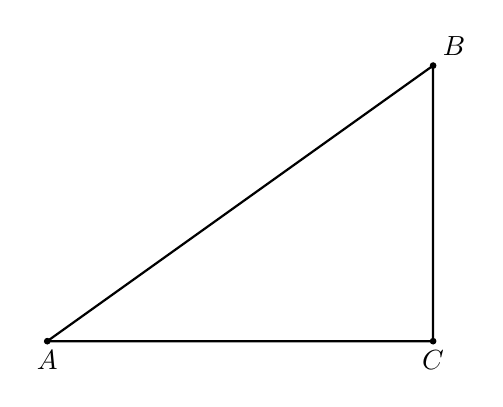
\begin{tikzpicture}[scale=0.7]
          \draw [thick](-1,0)--(6,0)--(6,5)--cycle;
          \draw [fill] (-1,0) circle [radius=0.05] node[below]{$A$};
          \draw [fill] (6,0) circle [radius=0.05] node[below]{$C$};
          \draw [fill] (6,5) circle [radius=0.05] node[above right]{$B$};
        \end{tikzpicture}
      \end{flushright}
  
\item Given right $\triangle JKL$ with $\overline{JK} \perp \overline{KL}$, $JK=20$, $m\angle J=11^\circ$. (mark the diagram)\\[0.5cm]
    Let $x$ be the length of the side opposite $\angle J$, $x=KL$. Write an equation expressing $\tan \angle J$ as a ratio of \emph{opposite} over \emph{adjacent}. \hfill (2 stars)
      \begin{flushright}
          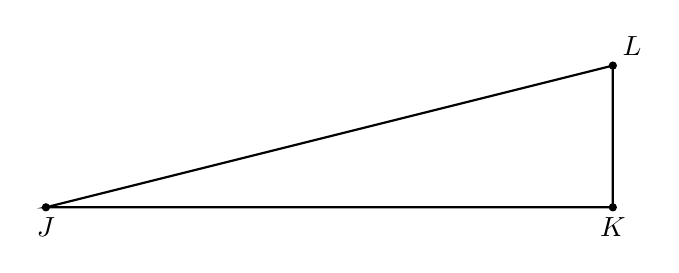
\begin{tikzpicture}[scale=0.9]
            \draw [thick](-1,0)--(7,0)--(7,2)--cycle;
            \draw [fill] (-1,0) circle [radius=0.05] node[below]{$J$};
            \draw [fill] (7,0) circle [radius=0.05] node[below]{$K$};
            \draw [fill] (7,2) circle [radius=0.05] node[above right]{$L$};
          \end{tikzpicture}
        \end{flushright}
\newpage
\subsubsection*{Mastery topic: Algebraic solution\\[0.5cm]
Use your calculator and solve each equation for $x$, rounding to the nearest tenth.}
\item $\displaystyle \tan 75^\circ = \frac{x}{15}$ \hfill (2 stars) \vspace{3cm}
\item $\displaystyle \tan 26^\circ = \frac{4}{x}$ \hfill (3 stars) \vspace{4cm}
\item $\displaystyle x = \tan^{-1} (\frac{2}{3.5})$ \hfill (2 stars) \vspace{3cm}
\item $\displaystyle \tan x^\circ = \frac{17}{9}$ \hfill (3 stars) \vspace{3cm}


\end{enumerate}
\end{document}